\documentclass[12pt,a4paper]{scrreprt}

\usepackage{graphicx}
\usepackage{a4}
\usepackage[ngerman]{babel}
\usepackage[utf8]{inputenc}
\usepackage{hyperref}
\usepackage[nottoc,notindex,notlot]{tocbibind}
\usepackage{nameref}
\usepackage{subcaption}
\usepackage{listings}
\usepackage{color}
\usepackage{xcolor}
\usepackage{longtable}
\usepackage{amsmath}
\usepackage{scrhack}
\usepackage{mathabx}

\lstdefinestyle{MyCodeStyle}{
	belowcaptionskip=1\baselineskip,
	breaklines=true,
	frame=single,
	captionpos=b,
	numbers=left,
	xleftmargin=\parindent,,
	showstringspaces=false,
	basicstyle=\footnotesize\ttfamily,
	keywordstyle=\bfseries\color{green!40!black},
	commentstyle=\itshape\color{purple!40!black},
	identifierstyle=\color{blue},
	stringstyle=\color{orange}
}
\lstset{escapechar=@,style=MyCodeStyle}

\newcommand{\includecode}[3]{\lstinputlisting[label=#1,caption=#2,float=ht,aboveskip=0pt,belowskip=0pt]{#3}}
\newcommand{\absatz}{\\[12pt]}

\newcommand{\heute}{\the\day.\the\month.\the\year}
\newcommand{\thema}{Parallelisierter Genetischer Algorithmus für das TSP}
\newcommand{\abgabedatum}{\heute}
\newcommand{\autorTitel}{Timo Bertsch\\Joram Markert\\Fabian Meyer}
\newcommand{\autorAbs}{Timo Bertsch\\ & Joram Markert\\ & Fabian Meyer}
\newcommand{\studiengang}{Master Computer Science}
\newcommand{\prueferA}{Prof. Dr. Lutz Köhler}
\newcommand{\prueferB}{Pascal Schönthier}

\newcommand{\zusammenfassung}{Dieses Dokument stellt einen genetischen Algorithmus zur Lösung des Travelling-Salesman-Problems (kurz TSP) vor. Der Fokus liegt in dieser Implementierung jedoch nicht auf der logischen Optimierung der Laufzeit des Algorithmus, sondern in einem hohen Grad an Parallelisierung und maximaler Nutzung der zur Verfügung stehenden Ressourcen. Hierbei werden neben dem Parallelisierungsschritt und den Messergebnissen, sowohl das TSP selbst als auch die allgemeine Umsetzung eines genetischen Algorithmus für das TSP vorgestellt. Dieses Projekt wurde im Rahmen der Veranstaltung \textit{Architektur verteilter Systeme} der TH Köln entwickelt.}

\begin{document}

\begin{titlepage}

\vspace*{-3.5cm}

\begin{flushleft}
\hspace*{-1cm} 
\includegraphics[width=3.5cm]{thkoeln-logo}
\end{flushleft}

\vspace{2.5cm}

\begin{center}
	\huge{
		\textbf{\thema} \\[4.5cm]
	}
	\Large{
		\textbf{\autorTitel}} \\[1.5cm]
		\large{
		\textbf{\studiengang} \\[8cm]
	}
	\large{
		\textbf{Gummersbach, \abgabedatum} \\[2.3cm]
	}
\end{center}

\end{titlepage}

\pagenumbering{arabic}

\begin{center}
{\Large \textbf{Abstract}}
\end{center}

\bigskip

\begin{center}
	\begin{tabular}{p{2.8cm}p{10cm}}
		Thema: & \thema \\
		 & \\
		Author: & \autorAbs \\
		 & \\
		Prüfer: & \prueferA  \\[.5ex]
		 &  \prueferB \\
		 & \\
		Datum: & \abgabedatum \\
		 & \\
	\end{tabular}
\end{center}

\bigskip

\noindent
\zusammenfassung
\tableofcontents

\setlength{\parindent}{0pt}

\chapter{Einleitung}
\label{chap:einleitung}

Ziel des Moduls \textit{Architektur verteilter Systeme} war die Parallelisierung eines Algorithmus, der ein Problem löst. Es sollten die vorhandenen zehn Computer zur Lösung genutzt werden. Das Problem, welches der Algorithmus lösen sollte, war frei wählbar. In diesem Projekt wurde das \textit{Travelling-Salesman-Problem} (kurz TSP) gewählt (siehe \autoref{chap:tsp}), welches mit einem \textit{genetischen Algorithmus} gelöst werden sollte (siehe \autoref{chap:algorithmus}). Durch die Aufgabenstellung war das Projekt dazu konzipiert, keine logischen Optimierungsverfahren zu verfolgen. Stattdessen lag das Hauptaugenmerk auf der Entwicklung eines Algorithmus, der erst mit viel Rechenleistung, Zeit und einem hohen Grad an Parallelisierung immer bessere Ergebnisse liefern sollte.\absatz
Ziel des Projekts ist neben dem Generieren möglichst perfekter Lösungen für das TSP auch das Gewinnen neuer Erkenntnisse im Bereich der parallelen Programmverarbeitung. Die Ausarbeitung beginnt mit der Erörterung des Traveling-Salesman-Problems. Nachdem die Problematik vergegenwärtigt wurde, folgt im nachfolgenden Kapitel der Lösungsansatz: Der Genetische Algorithmus. In \autoref{chap:testumgebung} und \autoref{chap:technologie} wird auf die Test- und Entwicklungsumgebung sowie die verwendeten Technologien eingegangen. Die Ausarbeitung schließt mit den gewonnen Ergebnissen in \autoref{chap:auswertung} und einem Ausblick in \autoref{chap:ausblick} ab.\absatz
Diese Ausarbeitung ist die erläuternde Dokumentation zum Projektrepository. Zum besseren Verständnis empfiehlt es sich, das Projekt im Zusammenhang mit der Ausarbeitung auf der Versionverwaltungtungsplattform Github nachzuvollziehen. Bei dem Projektrepository wurde insbesondere Wert auf klare Strukturen und verständlichen Quelltext gelegt.  \footnote{\url{https://github.com/AvS2016/ParallelTSP} [Zugriff: \heute]}

\chapter{Das Travelling-Salesman-Problem}
\label{chap:tsp}

Das Traveling-Salesman-Problem (TSP, zu deutsch auch häufig "Problem des Handlungsreisenden" genannt) gehört zu den bekanntesten aller kombinatorischen Probleme. Das Problem behandelt den Wunsch eines Fischers, alle Häfen dieser Welt zu besuchen und zwar in möglichst kurzer Zeit (logischer Rückschluss: möglichst kurze Strecke). Die Grundbedingungen der Reise sind, dass kein Hafen doppelt besucht werden soll und der Fischer sich am Ende der Reise wieder im selben Hafen befinden möchte, in dem er diese auch begonnen hat (vgl. \cite{groetschel05}).\absatz
Das Traveling-Salesman-Problem ist das am intensivsten untersuchte kombinatorische Optimierungsproblem. Die Problematik beim TSP liegt in der Vielzahl der Möglichkeiten. Bei einer überschaubaren Anzahl von Knoten, die besucht werden sollen, ist es möglich, die optimale Route zu finden (vgl. \cite{groetschel05}). Anhand des folgenden Beispiels (\autoref{fig:tsp-sample}) kann dies veranschaulicht werden. Gegeben ist Deutschland mit 20 Städten. 
\pagebreak

\begin{figure}[ht]
  	\centering
	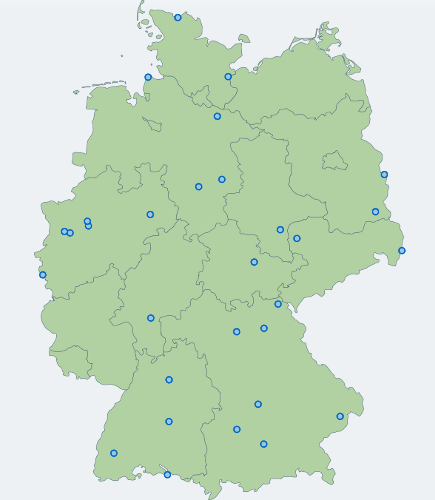
\includegraphics[width=300pt]{images/tsp_sample.png}
	\caption{TSP Beispielgraph\protect\footnotemark}
	\label{fig:tsp-sample}
\end{figure}
\footnotetext{\url{https://www-m9.ma.tum.de/games/tsp-game/index_de.html} [Zugriff: 20.09.2016]}

Alle Knoten (Städte) müssen mit Kanten (zurückgelegter Weg) verbunden werden, wobei keine Knoten mehrfach verbunden werden dürfen. Bei einer so üb"-er"-sch"-au"-bar"-en Problematik lässt sich die Möglichkeit mit geringem Aufwand auch durch menschliche Denkleistung finden. Optimale TSP Lösungen besitzen keine sich kreuzenden Kanten und verbinden die Knoten immer so, dass die Lösungswege eine konvexe Fläche bilden (vgl. \cite{groetschel05}).\absatz
Wie in \autoref{fig:tsp-sample-solved} zu sehen ist, verfügt die optimale Lösung über genau diese Eigenschaften. Bei c Problemen mit einer hohen Anzahl an Knoten ist -- sofern das Problem grafisch darstellbar ist -- für den Menschen leicht zu erkennen, ob es sich um eine gute oder weniger gute Lösung handelt, indem man eine Überprüfung der überschneidenden Kanten vornimmt. Allerdings ist es ab einer gewissen Komplexität nicht mehr möglich zu bestimmen, ob die gegebene Lösung wirklich die optimale ist.
\pagebreak

\begin{figure}[ht]
  	\centering
	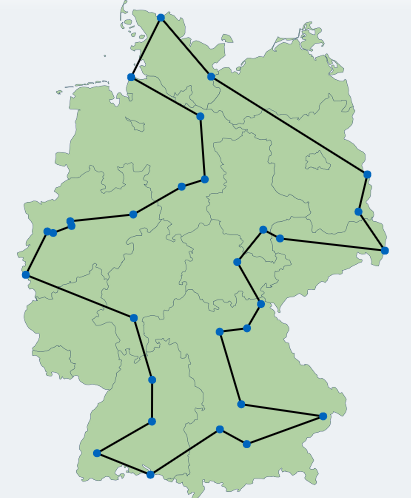
\includegraphics[width=300pt]{images/tsp_sample_solved.png}
	\caption{Optimale Lösung TSP Beispielgraph\protect\footnotemark}
	\label{fig:tsp-sample-solved}
\end{figure}
\footnotetext{\url{https://www-m9.ma.tum.de/games/tsp-game/index_de.html} [Zugriff: 20.09.2016]}

Es gibt $\frac{(n-1)!}{2}$ mögliche Lösungen, vorausgesetzt der Graph ist symmetrisch (vgl. \cite{groetschel05}). Das entspricht in diesem Fall bei 20 Städten 60.822.550.204.416.000 möglichen Lö"-su"-ng"-en. \autoref{tbl:tsp-is-huge} veranschaulicht die exponentielle Steigerung der möglichen Kombinationen.
\pagebreak

\begin{center}
\begin{longtable}{p{2.5cm} | p{6.5cm} }
Knoten & Mögliche Lösungen  \\
\hline
 & \\
10 & $181.440 $ \\
 & \\
50 & $ 3.04140932*10^{62} $ \\
 & \\
100 & $ 4.666310772*10^{155} $ \\
 & \\
1000 & $ 2.011936300*10^{2564} $ \\

\caption{Beispiel der kombinatorischen Explosion der TSP}
\label{tbl:tsp-is-huge}
\end{longtable}
\end{center}

Möchte man die optimale Route eines komplexen TSP ermitteln, muss man zu anderen Methoden als einem einfachen Brute-Force Ansatz greifen. Im Fall dieser Ausarbeitung wird ein Genetischer Algorithmus eingesetzt, um das Problem möglichst optimal und hochgradig parallelisiert auf einem Rechencluster zu lösen.

\chapter{Der Genetische Algorithmus}
\label{chap:algorithmus}

Im Rahmen dieses Projektes wurde ein Genetischer Algorithmus entwickelt, mit dem das TSP gelöst wird. Genetische Algorithmen werden im Allgemeinen zur Lösungsfindung bei komplexen Suchproblemen verwendet, bei denen eine kombinatorische Explosion vorliegt und der Lösungsraum so groß ist, dass eine Lösung mit einer optimalen Brute-Force-Methode nicht möglich ist.\absatz
Die allgemeine Funktionsweise dieses Algorithmus und die Variante, die in diesem Projekt entwickelt wurde, werden in \autoref{sec:funktionsweise} erläutert. Der Basisalgorithmus ist jedoch nicht nebenläufig konzipiert, daher mussten einige Modifikationen vorgenommen werden, um diesen in einem verteilten System einsetzen zu können. Diese Änderungen werden in \autoref{subsec:exchange} näher beschrieben.

\section{Funktionsweise}
\label{sec:funktionsweise}

Genetische Algorithmen basieren auf der Idee der natürlichen Auslese und ermitteln durch Selektion, Kombination und Evolution von möglichen Lösungen eine sehr gute bis perfekte Lösung für das gesuchte Problem.\\
Eine Lösung des gegebenen Problems wird als \textit{Individuum} bezeichnet. Im Rahmen des TSP sind Individuen Wege, die die Lösungskriterien des TSP erfüllen (siehe \autoref{chap:tsp}). Die Knoten, die bei einer Lösung besucht werden, werden als \textit{Eigenschaften} oder \textit{Gene} eines Individuums bezeichnet. Eine Menge von Individuen, auf der der Algorithmus operiert, wird \textit{Population} genannt. Der Genetische Algorithmus arbeitet iterativ in Schritten, die als \textit{Generationen} bezeichnet werden. Die Individuen einer Population werden schrittweise in diesen \textit{Generationen} mit einer \textit{Fitness} bewertet, aussortiert und rekombiniert, um die Qualität der Lösungen zu verbessern. Die Phasen einer Generation werden in \autoref{tbl:phasen-algorithmus} zusammenfassend dargestellt (vgl. \cite{jacobsen12A}).
\pagebreak
\begin{center}
\begin{longtable}{p{3.0cm} p{10cm}}

Phase & Beschreibung \\
\hline \\
\textit{Initialisierung} & Die initiale Population wird generiert. Dieser Schritt wird nur ein einziges Mal zu Beginn des Algorithmus ausgeführt. Die Population wird mit zufällig generierten Individuen erstellt.\\
 & \\
\textit{Evaluation} &  Die Individuen der aktuellen Generation werden mit einem Fitnesswert bewertet. Dieser Zahlenwert drückt aus, wie gut das Individuum bzw. die Lösung des Problems ist. In Bezug auf das TSP bedeutet eine kürzere Strecke der Lösung eine höhere Fitness des entsprechenden Individuums.\\
 & \\
\textit{Selektion} & Aus den Individuen der aktuellen Generation werden diejenigen ausgewählt, die für die Crossover Phase verwendet und die in die nächste Generation übernommen werden. Hierbei ist es von zentraler Bedeutung, dass Individuen mit hoher Fitness mit einer höheren Wahrscheinlichkeit ausgewählt werden als Individuen mit niedriger Fitness.\\
 & \\
\textit{Crossover} & Aus den ausgewählten Individuen (sog. Eltern) werden durch die Kombination von deren Eigenschaften neue Individuen (sog. Kinder) erzeugt, die in die nächste Generation übernommen werden. In Bezug auf das TSP werden hier Teilwege der Eltern so miteinander kombiniert, dass die Kinder wieder eine valide Lösung des TSP darstellen.\\
 & \\
\textit{Mutation} & Die Gene der erzeugten Kinder werden per Zufall verändert, um eine Stagnation des Genpools zu verhindern und neue Lösungsmöglichkeiten zu erzeugen. Diese Stagnation kann auftreten, wenn über mehrere Generationen hinweg besonders fitte Individuen die Population dominieren.\\

\caption{Phasen des genetischen Algorithmus}
\label{tbl:phasen-algorithmus}
\end{longtable}
\end{center}

Die Umsetzung dieser Phasen im Rahmen dieses Projekts wird in den folgenden Unterabschnitten anhand des Beispielgraphen in \autoref{fig:algo-sample} detailliert beschrieben.

\begin{figure}[ht]
  	\centering
	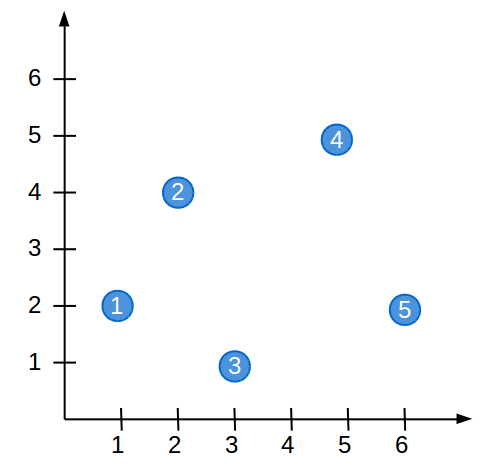
\includegraphics[width=400pt]{images/algo_01_sample.png}
	\caption{Beispielgraph}
	\label{fig:algo-sample}
\end{figure}

Dieses Beispiel zeigt einen Graphen mit fünf Knoten, die jeweils durch die Nummer in ihrer Mitte identifiziert werden können.

\subsection{Initialisierung}
\label{subsec:initialisation}

Die \textit{Initialisierungsphase} wird nur einmal zu Beginn des Algorithmus ausgeführt. In dieser Phase wird die initiale Population generiert, mit der der Algorithmus dann arbeitet. Die Individuen werden hierbei vollständig zufallsgeneriert, wobei jedes Individuum eine valide Lösung des TSP darstellt. Dieser Vorgang wird in \autoref{lst:algo-generierung} dargestellt.

\includecode{lst:algo-generierung}{Generierung eines Individuums}{code/algo_01_generierung.txt}

Um ein Individuum zu generieren, wird eine Liste (\textit{nodes}) aller Knoten innerhalb des gegebenen Graphen für das Individuum erstellt (Z. 1). Aus dieser Liste wird dann ein Knoten zufällig ausgewählt (Z. 5) und dem Individuum hinzugefügt (Z. 6). Danach wird der Knoten aus der Liste der übrigen Knoten entfernt (Z. 7) und dieser Prozess wird solange wiederholt bis keine Knoten mehr in der Liste \textit{nodes} vorhanden sind (Z. 4).\absatz
Mit diesem Verfahren können die in \autoref{fig:algo-sample-individuals} dargestellten Individuen aus dem Beispielgraphen in \autoref{fig:algo-sample} generiert werden.

\begin{figure}[ht]
  	\centering
	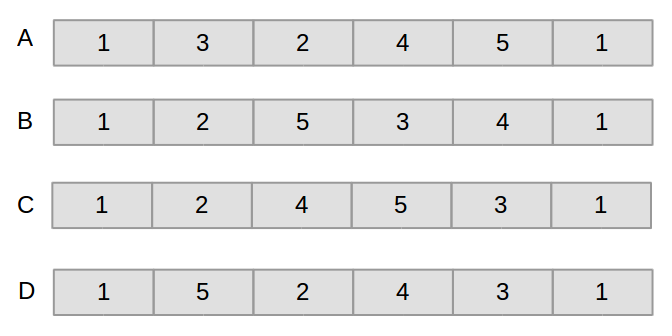
\includegraphics[width=400pt]{images/algo_02_init.png}
	\caption{Beispiel: Zufällig generierte Individuen}
	\label{fig:algo-sample-individuals}
\end{figure}

\subsection{Evaluation}
\label{subsec:evaluation}

In der \textit{Evaluationsphase} werden die Individuen der Population der aktuellen Generation bewertet und damit ihr Fitnesswert errechnet. Jedes Individuum stellt einen Weg durch den Graphen, also eine Liste aufeinander folgender Knoten, dar. Die Fitness errechnet sich aus der Länge dieses Weges. Diese Länge wird durch die Summe des euklidischen Abstands zwischen in der Liste aufeinanderfolgenden Knoten beschrieben, wie in der folgenden Gleichung dargestellt wird.

$$
l_{individuum} = \sum_{i=1}^{n} \sqrt{(x_{i+1} - x_i)^2 + (y_{i+1} - y_i)^2}
$$

Hierbei stellt $l_{individuum}$ die Distanz des Lösungsweges des entsprechenden Individuums dar. $n$ ist die Anzahl aller Knoten, die das Individuum umfasst. $x_i$, $x_{i+1}$, $y_i$ und $y_{i+1}$ sind die Koordinaten des Knoten $i$ bzw. $i+1$.\\
Dies wird für alle Individuen wiederholt. Hierbei gilt, dass je länger der Weg ist, desto niedriger ist der Fitnesswert eines Individuums. Damit verhält sich die Fitness also \textit{antiproportional} zur Länge des Weges.\\
Aufgrund von Rundungsfehlern bei Gleitkommazahlen reicht ein einfacher Kehrwert der Länge des Weges nicht aus, um die Fitness eines Individuums zu berechnen, da der Weg je nach Größe des Graphen entsprechend lang werden kann. Daher wird aus allen Individuen der aktuellen Population dasjenige gesucht, das den längsten Weg $l_{max}$ besitzt. Mit diesem Wert wird nun die Fitness $f_{individuum}$ jedes Individuums auf folgende Weise berechnet.

$$
f_{individuum} = \frac{l_{max}}{l_{individuum}}
$$

\autoref{tbl:algo-sample-fitness} zeigt die Weglänge und die Fitness der Individuen aus \autoref{fig:algo-sample-individuals}.

\begin{center}
\begin{longtable}{p{2.5cm} | p{6.5cm} | p{3.0cm}}
Individuum & $l_{individuum}$ & $f_{individuum}$ \\
\hline & & \\
A & $1 + \sqrt{10} + \sqrt{10} + \sqrt{10} + 5 = 15.49$ & $\frac{19.34}{15.49} = 1.25$ \\
& & \\
B & $\sqrt{5} + \sqrt{20} + \sqrt{10} + \sqrt{20} + 5 = 19.34$ & $\frac{19.34}{19.34} = 1$ \\
& & \\
C & $\sqrt{5} + \sqrt{10} + \sqrt{10} + \sqrt{10} + 1 = 12.72$ & $\frac{19.34}{12.72} = 1.52$ \\
& & \\
D & $5 + \sqrt{20} + \sqrt{10} + \sqrt{20} + 1 = 18.11$ & $\frac{19.34}{18.11} = 1.07$\\

\caption{Beispiel Fitness und Distanz}
\label{tbl:algo-sample-fitness}
\end{longtable}
\end{center}

\subsection{Selektion}
\label{subsec:selection}

Während der \textit{Selektionsphase} werden die Individuen (Eltern) ausgewählt, aus denen die Individuen für die nächste Generation (Kinder) generiert werden. Die Auswahl geschieht anhand der Fitness der Individuen. Wichtig ist hierbei auch, dass ein einzelnes Individuum mehrfach ausgewählt werden kann.\\
In diesem Projekt wurde zur Auswahl der Eltern das \textit{Roulette-Wheel-Verfahren} verwendet. Bei diesem Verfahren werden die Individuen durch eine Zufallszahl ausgewählt, wobei jedoch besonders fitte Individuen eine besonders hohe Chance haben ausgewählt zu werden. Hierbei wird die Fitness der Individuen auf das Intervall [0;1] normiert. Daraufhin wird ein \textit{Auswahlintervall} für jedes Individuum berechnet, indem beim Durchlauf der Liste der Individuen, die entsprechend der Fitness der Individuen sortiert ist, pro Individuum die Fitness aller voranstehenden Individuen aufsummiert wird. Der sich daraus ergebende Wert ist die untere Grenze $g_{x unten}$ des Auswahlintervalls des Individuums $x$. Die obere Grenze $g_{x oben}$ wird durch die Summe aus unterer Grenze und der Fitness des aktuellen Individuums gebildet (vgl. \cite{rongqu14}). Die folgenden Gleichungen beschreiben den Rechenweg nochmals.

$$
g_{x unten} = \sum_{i=1}^{i<x} f_i
$$
$$
g_{x oben} = g_{x unten} + f_x
$$

\autoref{fig:algo-sample-interval} zeigt die Auswahlintervalle der Individuen aus \autoref{fig:algo-sample-individuals}.

\begin{figure}[ht]
  	\centering
	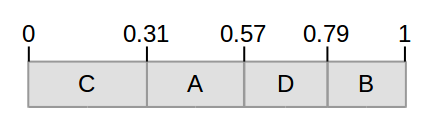
\includegraphics[width=300pt]{images/algo_03_interval.png}
	\caption{Beispiel: Auswahlintervalle der Individuen}
	\label{fig:algo-sample-interval}
\end{figure}

Nun wird eine Zufallszahl im Intervall [0;1] gewürfelt und es wird dasjenige Individuum zum Elternteil erwählt, in dessen Intervall die Zufallszahl fällt. Dabei werden immer Paare von zwei Eltern gebildet, aus denen ein neues Individuum generiert wird. Dies wird solange wiederholt bis genügend Individuen ausgewählt wurden, um die aktuelle Population vollständig zu ersetzen.\absatz
Zusätzlich zur Auswahl der Individuen verwendet der Algorithmus außerdem eine \textit{Elitism} Mechanik, durch die die besten Individuen der aktuellen Generation in die nächste Generation übernommen werden. So wird verhindert, dass bereits gefundene sehr gute Lösungen wieder verworfen werden. Alle anderen Individuen der aktuellen Generation werden jedoch durch neue Individuen, die Kinder, ersetzt.

\subsection{Crossover}
\label{subsec:crossover}

In der \textit{Crossoverphase} werden die aus der \textit{Selektionsphase} aus"-ge"-wähl"-ten Eltern kombiniert, um neue Individuen für die nächste Generation zu generieren.\\
Hierbei wird ein zusammenhängender Teilweg des El"-tern"-indi"-vid"-uums A zu"-fä"-llig ausgewählt und genau so in das Kind E übernommen. Um die restlichen Knoten des Kindes zu füllen, werden der Reihe nach Knoten aus Elternindividuum B entnommen, falls diese in dem Kind noch nicht vorhanden sind, und in das Kind eingefügt (vgl. \cite{jacobsen12B}). In \autoref{fig:algo-sample-crossover} wird dieser Prozess nochmal verdeutlicht.

\begin{figure}[ht]
	\centering
	\begin{subfigure}[t]{400pt}
    	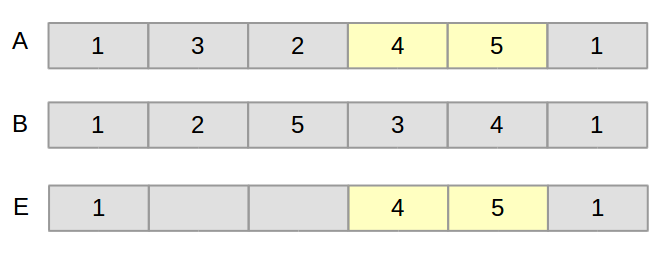
\includegraphics[width=400pt]{images/algo_04_crossover_1.png}
        \caption{}
        \label{fig:algo-sample-crossover1}
    \end{subfigure}

    \begin{subfigure}[t]{400pt}
    	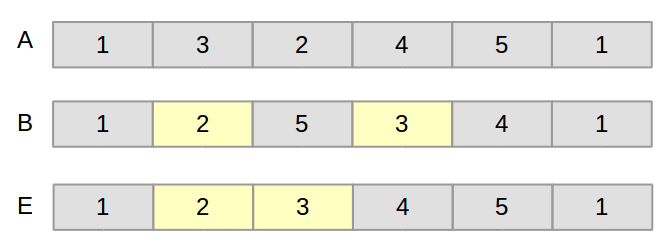
\includegraphics[width=400pt]{images/algo_04_crossover_2.png}
        \caption{}
        \label{fig:algo-sample-crossover2}
    \end{subfigure}

	\caption{Beispiel: Crossover von zwei Individuen}
	\label{fig:algo-sample-crossover}
\end{figure}

In \autoref{fig:algo-sample-crossover1} wurde der Teilweg [4,5] aus Individuum A ausgewählt und an der gleichen Stelle in das neue Kind E eingefügt. Im nächsten Schritt werden in \autoref{fig:algo-sample-crossover2} die Knoten in Individuum B der Reihe nach durchgegangen und, falls sie in Individuum E noch nicht vorhanden sind, entsprechend eingefügt.\\
Das neu entstandene Individuum E ist nun eine Kombination aus den Lösungen von A und B und umfasst ohne weitere Korrekturen immer direkt eine valide Lösung des TSP.\\
Dieser Vorgang wird nun für alle im \textit{Selektionsschritt} ausgewählten Elternpaare wiederholt.

\subsection{Mutation}
\label{subsec:mutation}

Die \textit{Mutationsphase} dient dazu, um die Variation im Genpool der Population aufrecht zu erhalten. So kann es passieren, dass ein besonders fittes Individuum die Selektionsphase dominiert und der Genpool gegen diese Lösung konvergiert. Durch die genetische Verarmung können potentiell bessere Lösungen nicht mehr gefunden werden (vgl. \cite{rongqu14}). Um diesem Effekt entgegenzuwirken, wird ein sehr kleiner Anteil aller Kinder, die im \textit{Crossover} Schritt generiert wurden, zufällig mutiert.\\
Im Rahmen dieses Projekts wurde die \textit{Swap Mutation} verwendet, um Individuen zu mutieren. Hierbei werden zwei zufällig ausgewählte Knoten aus einem Individuum miteinander vertauscht. Die hieraus entstandene Lösung ist ebenfalls wieder eine valide Lösung des TSP (vgl. \cite{jacobsen12B}). \autoref{fig:algo-sample-mutation} zeigt diesen Vorgang nochmals anhand des in \autoref{subsec:crossover} erzeugten Individuums E.


\begin{figure}[ht]
  	\centering
	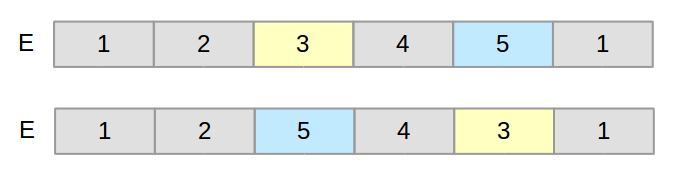
\includegraphics[width=400pt]{images/algo_05_mutation.png}
	\caption{Beispiel: Mutation eines Individuums}
	\label{fig:algo-sample-mutation}
\end{figure}

Hierbei werden per Zufall die beiden Knoten 3 und 5 ausgewählt. Deren Position in der Liste wird daraufhin einfach vertauscht, wodurch die Lösung unter Umständen völlig neue Möglichkeiten in die Population einbringt.

\subsection{Exchange}
\label{subsec:exchange}

Die bisher vorgestellten Phasen beschreiben einen Genetischen Algorithmus aus dem Lehrbuch, der rein single threaded funktioniert. Um diesen Algorithmus nun zu parallelisieren, wird er um eine weitere Phase erweitert.\\
Die Problematik beim TSP ist, dass die Komplexität des Lösungsraumes exponentiell mit der Größe des verwendeten Graphen steigt (siehe \autoref{chap:tsp}). Um das TSP für größere Graphen mit einem Genetischen Algorithmus zu lösen, muss die Größe der verwendeten Population vergrößert werden, damit die Population allein durch die schiere Anzahl an Lösungsmöglichkeiten nicht genetisch verhungert. Jedoch benötigen größere Populationen deutlich mehr Rechenleistung pro Generation, sodass sehr große Graphen nur langsam gelöst werden können.\\
Um diese Problematik zu lösen, wurde die Population auf mehrere Prozesse verteilt. Jeder dieser Prozesse ist single threaded und berechnet den Genetischen Algorithmus gemäß den bereits vorgestellten Phasen vollständig unabhängig von den anderen Prozessen. Am Ende jeder Generation treten jedoch alle Prozesse in die \textit{Exchangephase} ein. In dieser Phase senden alle Prozesse einen Anteil von 10\% ihrer Population an einen anderen Prozess. Der sendende Prozess löscht diese Individuen aus seiner Population und der empfangende Prozesse fügt die erhaltenen Individuen in seine Population ein. Hierzu müssen alle Prozesse die gleiche Populationsgröße besitzen, sodass nach dem Austausch die Population wieder gleich groß ist wie zuvor. Durch diesen Austausch von Individuen entsteht ein Austausch von Genmaterial, sodass die verschiedenen Populationen der Prozesse näherungsweise wie eine einzige große Population funktionieren. So agieren 10 Prozesse mit einer Population von 1000 Individuen so wie ein einziger Prozess mit 10000 Individuen. Darüber hinaus kann jeder Prozess die rechenintensiven Phasen auf einem separaten Kern mit einer Populationsgröße von 1000 statt 10000 ausführen, sodass die Prozessgemeinschaft abzüglich des Kommunikationsoverheads näherungsweise so schnell abläuft, wie ein einzelner Prozess mit nur 1000 Individuen.\\
In \autoref{fig:algo-sample-exchange} ist zu sehen, wie der Austausch der Individuen mit fünf Prozessen funktioniert.

\begin{figure}[ht]
  	\centering
	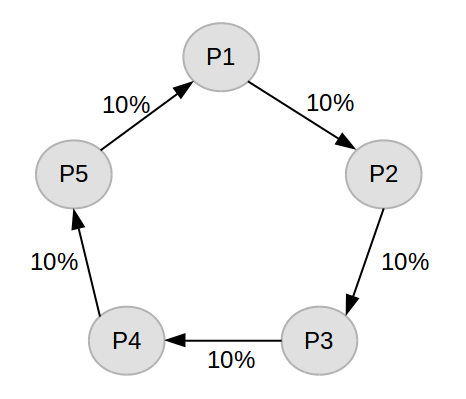
\includegraphics[width=300pt]{images/algo_06_exchange.png}
	\caption{Beispiel: Austausch der Individuen}
	\label{fig:algo-sample-exchange}
\end{figure}

Hierbei wird ein Ringaustauschverfahren verwendet. Jeder Prozess hat eine eindeutige ID und gibt seine Individuen an den jeweils nächsten Prozess weiter, also P1 sendet an P2, P2 an P3, usw. Dadurch wird ein kompliziertes Kommunikationsverfahren zur Findung von Partnerprozessen vermieden und der Netzwerkoverhead wird möglichst gering gehalten.

\chapter{Test- und Entwicklungsumgebung}
\label{chap:testumgebung}

Für die Umsetzung und Test dieses Projektes stand das Labor für Prozessinformatik am Campus Gummersbach zur Verfügung. Dort befinden sich zehn Apple Desktoprechner, welche jeweils mit zwei Vier-Kern-Prozessoren ausgestattet und über ein Gigabit Ethernet Netzwerk verbunden sind. Dieser Aufbau lässt sich somit auch als Cluster bezeichnen. Die Prozessoren von sechs der zehn Rechner unterstützen zudem Hyper-Threading und sind dadurch leistungsfähiger als die restlichen vier.\absatz
Da keiner der Autoren über einen Apple-Rechner verfügt, entschied sich das Team für eine Entwicklung unter Ubuntu-Linux aufgrund der ähnlichen Systemarchitektur von Mac OS X und Linux.\\
Im folgenden Kapitel werden die konkrete Realisierung des Projektes und die dazu verwendeten Technologien beschrieben.

\chapter{Technologie}
\label{chap:technologie}

In diesem Kapitel wird erläutert, welche Technologien, warum und wie für dieses Projekt eingesetzt wurden.

\section{Programmiersprache}
\label{sec:programmiersprache}

Zu Beginn des Projektes wurden zunächst Vorschläge durch das Team gesammelt, welche Programmiersprachen für die Lösung und Umsetzung der Problematik in Frage kommen würden. Zur Diskussion standen schließlich \textit{C++}, \textit{C\#}, \textit{Python} und \textit{Rust}. Bei der Wahl der Programmiersprache waren die folgenden Aspekte wichtig: Zum einen sollte die Programmiersprache einem Teammitglied zumindest in den Grundlagen bekannt sein, um einen auf Implementierung und Technologie fokussierten Arbeitsablauf zu gewährleisten. Darüber hinaus gab es im Team keine vorherigen Erfahrungen im Aufbau und Umgang mit parallelen Programmen über mehrere Rechner hinweg. Aus diesem Grund wurde der Lernfokus auf die Parallelisierung der Anwendung gelegt und nicht in das Erlernen neuer Programmiersprachen. Zudem beeinflussten sich die Entscheidungen für die Wahl einer Programmiersprache und die Wahl der Technologie für die Interprozesskommunikation gegenseitig. Eine genauere Erläuterung dazu folgt im nächsten Abschnitt. Ein weiterer wichtiger Punkt war, dass der Quelltext ohne großen Aufwand sowohl auf Linux als auch auf Mac OS X ausführbar ist, da keiner aus dem Team die Möglichkeit hatte direkt unter Mac OS X zu entwickeln.\\
Die Programmiersprache \textit{Rust} wurde ausgeschlossen, da es innerhalb des Teams an Erfahrung im Umgang damit mangelte und es aufgrund des geringen Alters der Sprache (zum Zeitpunkt der Entwicklung dieses Algorithmus) vergleichsweise wenig Bibliotheken und nur eine kleine Community gab.\\
Da es sich bei \textit{Python} um eine Skriptsprache handelt, wurde aus Performanzgründen schließlich entschieden, dass auch diese nicht für Umsetzung des Projekts in Frage kommt.\\
Bei \textit{C\#} wäre die Verwendung von \textit{Mono} als plattformübergreifende Implementierung für .NET notwendig gewesen, um auch unter OS X und Linux lauffähig zu sein. Da auch damit im Team noch keine Erfahrungen vorhanden waren, fiel die Entscheidung letztendlich C++ zu.\\
Für C++ gibt es Compiler sowohl unter Linux, Mac OS X als auch für Windows. Zudem gab es für jede der zur Wahl stehenden Technologien der Interprozesskommunikation entsprechende Bibliotheken. So entschieden wir uns schließlich für C++ als Programmiersprache.

\section{Interprozesskommunikation}
\label{sec:interprozesskommunikation}

Damit die einzelnen Prozesse verteilt auf mehrere Prozessorkerne bzw. verteilt auf mehrere Rechner, Daten miteinander austauschen können, ist die Wahl eines geeigenten Protokolls notwendig. Zur Diskussion standen MQTT (MQ Telemetry Transport) und MPI (Message Passing Interface). Bei MQTT handelt es sich um ein leichtgewichtiges Protokoll mit einem Publish-Subscribe-Mechanismus, wohingegen MPI deutlich komplexer ist. Auf der Webseite von boost \footnote{\url{http://www.boost.org/doc/libs/1_60_0/doc/html/mpi.html} [Zugriff: 15.9.2016]} wird MPI als die beliebteste Bibliothek für verteilte Hochleistungsanwendungen bezeichnet. Aufgrund der großen Verbreitung von MPI, entschied sich das Team dafür, dieses Protokoll näher kennenzulernen.\\
Im Folgenden wird auf die verwendeten Grundfunktionalitäten von MPI näher eingegangen.

\subsection{Daten senden und empfangen}
\label{subsec:daten_senden_und_empfangen}

MPI abstrahiert das zugrunde liegende Netzwerk, wodurch sich ein Entwickler nicht damit auseinandersetzen muss, wie die Informationen ausgetauscht werden (z.B. über Sockets, Shared Memory, Pipes, etc.). Die MPI-Implementierung realisiert den Datenaustausch automatisch über den am besten geeigneten Kanal, wodurch es für den Entwickler keine Rolle spielt, ob sich zwei Instanzen auf dem gleichen Rechner oder verteilt auf mehreren befinden. Sollen Daten von einem Prozess zu einem zweiten gesendet werden, so stehen dafür die Funktionen \lstinline$MPI_Send$ und \lstinline$MPI_Recv$ zur Verfügung. Die Identifikation einzelner Instanzen erfolgt über den von MPI zugewiesenen, eindeutigen \textit{Rank}. Dieser muss bei beiden Funktionen als Parameter angegeben werden. Bei \lstinline$MPI_Send$ als Ziel und bei \lstinline$MPI_Recv$ als Sender der Nachricht. Neben den zu übermittelnden Daten müssen außerdem der Datentyp, die Anzahl der Datenpakete, ein \textit{Tag} und der Kommunikator (\lstinline$MPI_Comm$) spezifiziert sein. In \autoref{lst:mpi_send_recv} sind die Funktionsaufrufe als C++ Code dargestellt.

\includecode{lst:mpi_send_recv}{Daten mit MPI senden und empfangen}{code/mpi_send_recv.cpp}

Eine andere Möglichkeit Daten auszutauschen, ist ein Broadcast, welcher mit dem Befehl \lstinline$MPI_Bcast$ ausgeführt werden kann. Dabei wird dann eine Nachricht an alle vorhandenen Prozesse gesendet.

\subsection{Prozesse auf mehreren Rechnern starten}
\label{subsec:prozessstart}

Um ein Programm parallel auf mehreren Rechnern ausführen zu können, mu"-ss die Software auf jedem Rechner gestartet werden. Es wäre sehr aufwändig, wenn dies überall manuell durchgeführt werden müsste.\\
In diesem Projekt wurde Open MPI als Implementierung für das Message-Passing-Interface verwendet. Sollen von einem Programm mehrere Instanzen erstellt werden, die mittels MPI Daten austauschen, so muss dieses Programm von MPI selbst gestartet werden. Open MPI wird gestartet, indem die Anwendung \textit{mpiexec} ausgeführt wird. Per SSH ist diese Anwendung zudem in der Lage, das Programm, welches von MPI gestartet werden soll, auch auf anderen Rechnern auszuführen. Dafür kann \textit{mpiexec} z.B. eine \textit{hostfile} als Parameter übergeben werden, welches für jeden gewünschten Rechner eine Zeile mit dessen Namen und der maximalen Anzahl an zur Verfügung stehenden Slots beinhaltet. Ein weiteres Argument legt den Pfad zu der auszuführenden Anwendung fest. Schließlich muss noch die Anzahl der zu startenden Prozesse angegeben werden, welche MPI dann automatisch auf die zur Verfügung stehenden Rechner verteilt.

\section{Versionsverwaltung, Build System und Tests}
\label{sec:versionsverwaltung}

Um den Softwareentwicklungsprozess weiter zu unterstützen, wurde ein Versionverwaltungssystem verwendet. Da die Mehrzahl der Teammitglieder bereits Erfahrung damit hatte, wurde \textit{Git} als Versionsverwaltungssystem und \textit{GitHub} als Plattfrom verwendet. \footnote{\url{https://github.com/AvS2016/ParallelTSP} [Zugriff: \heute]} Diese Oberfläche bietet zudem den Vorteil, dass Dateien auch direkt über den Browser eingesehen und bearbeitet werden können. Die Protokolle der Team-Meetings, sowie die daraus resultierenden Ergbenisse konnten somit direkt im Browser als Markdown-Dateien\footnote{\url{https://guides.github.com/features/mastering-markdown/} [Zugriff: 15.9.2016]} angelegt werden.\absatz
Weiterhin wurden Unit Tests eingeführt, um nach einer Änderung am Quellcode nicht sämtliche Funktionen erneut manuell testen zu müssen. Dafür kam das \textit{Catch} Framework
\footnote{\url{https://github.com/philsquared/Catch} [Zugriff: 15.9.2016]} zum Einsatz.\absatz
Um die Software nach jeder Änderung automatisch zu verifizieren, wurde eine Continuous Integration Infrastruktur mithilfe des Dienstes \textit{Travis CI} aufgebaut. \footnote{\url{https://travis-ci.org} [Zugriff: 15.9.2016]} Dazu wird unter GitHub ein Webhook für das entsprechende Repository eingerichtet, welcher dafür sorgt, dass Travis über jede Änderung des Repositorys benachrichtigt wird. Daraufhin erstellt Travis eine virtuelle Maschine, auf welcher der aktuelle Stand des Repositorys kopiert, kompiliert und ausgeführt wird. Die \textit{travis.yml} Datei des Projekts enthält entsprechende Anweisungen für den Continuous Integration Dienst, welche Abhängigkeiten das Projekt benötigt und wie es kompiliert werden soll. Anschließend werden die Unit Tests durchgeführt und in der \textit{README.md} auf GitHub angezeigt, ob der Build- und Testvorgang erfolgreich war oder fehlgeschlagen ist.\absatz
Um die Anwendung im Gesamten zu erstellen, wird CMake als Buildsystem verwendet. Dadurch ist nur ein Befehl notwendig, um die einzelnen Programmteile zu kompilieren. Die benötigten Informationen für die Programmerstellung bezieht CMake aus den \textit{CMakeList.txt}-Dateien, wobei für jeden Programmteil eine solche Konfiguration vorhanden ist.

\section{Nützliche Skripte}
\label{sec:nuetzliche_skripte}

Um das Projekt erstellen und ausführen zu können, werden einige Abhängigkeiten wie \textit{Open MPI, Boost} und \textit{Catch} benötigt. 
Da es sich gerade bei den ersten beiden um große Bibliotheken handelt, dauert die Installation einige Minuten. Damit alle Abhängigkeiten direkt nacheinander und vollautomatisch installiert werden können, wurden im Rahmen des projektes entsprechende Bash Skripte geschrieben.\\
So werden durch das Ausführen der Datei \textit{script/get-linux-deps.sh} die entsprechenden Anwendungen und Bibliotheken installiert. Die Skripte wurden unter Ubuntu 16.04, Debian 8 und Mac OS X getestet.\absatz
Als aufwändig erwies sich zudem die Verteilung der kompilierten Anwendungen auf alle Rechner im Cluster. Um dies zu vereinfachen, komprimiert das  Skript \textit{script/copy\_repo.sh} das Projektverzeichnis automatisch, verteilt diese auf alle Rechner im Cluster und entpackt diese dort wieder.

\section{Visualisierung des Graphen}
\label{sec:visualisierung_graph}

Um das Graphenproblem zu veranschaulichen, war eine visuelle Darstellung des Graphen wünschenswert. Die hierfür in Betracht gezogenen Möglichkeiten waren:

\begin{itemize}
\item Eine openGL Anwendung, welche den Graphen zwei- oder dreidimensional darstellen kann
\item Die Erstellung einer Vektorgraphik direkt aus der Graphdefinition
\item Zeichnen des Graphen mittels Gnuplot \footnote{\url{http://www.gnuplot.info/} [Zugriff: 20.9.2016]}
\item Zeichnen des Graphen mittels Matplotlib
\end{itemize}

Die Entscheidung gegen die Erstellung einer openGL Anwendung ist aufgrund des hohen Mehraufwandes gefallen. Zudem erschien es nicht notwendig, eine dreidimensionale Ansicht des Graphen zu haben. Bei der Betrachtung der verbleibenden Vorschläge, erwies sich auch die direkte Erstellung einer Vektorgraphik als umfangreicher, als Gnuplot zu verwenden, um die Liste der Punkte auszugeben. Außerdem lässt sich die Gnuplotausgabe unter anderem auch als Vektorgraphik speichern. Da bereits Erfahrung mit Gnuplot im Team vorhanden war, wurde auch Matplotlib schließlich ausgeschlossen.\\
Um aus einem Graphen mithilfe von Gnuplot eine Vektorgraphik zu erstellen, gibt es in diesem Projekt die Anwendung \textit{graphconv}. Ein Graph liegt immer in Form einer \textit{*.json}- Datei vor, deren Pfad die genannte Anwendung als Parameter erhält. Weitere Parameter sind ein Verweis auf den bereits ermittelten Pfad (ebenfalls in Form einer \textit{*.json}- Datei) sowie der Name der zu erstellenden Vektorgraphik. Daraufhin generiert \textit{graphconv} zwei neue Dateien. Die erste (\textit{*.dat}) enthält die Koordinaten aller Punkte des Graphen. Zwischen aufeinanderfolgenden Punkten gibt es jeweils eine Kante (definiert durch den Pfad, der sich in der zweiten übergebenen \textit{*.json}- Datei befindet), zudem ist per Definition der erste mit dem letzten Punkt identisch, sodass insgesamt ein geschlossener Graph entsteht. Die zweite Datei (\textit{*.plt}) enthält die Visualisierungsanweisungen für Gnuplot, wie beispielsweise Farbe und Größe der Punkte, die Einteilung der Achsen sowie den abschließenden Renderbefehl mit dem Verweis auf die \textit{*.plt}- Datei. Je nach Größe des Graphen variiert auch die Größe der gezeichneten Punkte und die Breite der Kanten. Die mit Gnuplot erstellte Ansicht, wie in \autoref{fig:gnuplot-sample} zu sehen, wird anschließend als Vektorgraphik in eine \textit{*.svg}- Datei gespeichert.
\pagebreak

\begin{figure}[ht]
  	\centering
	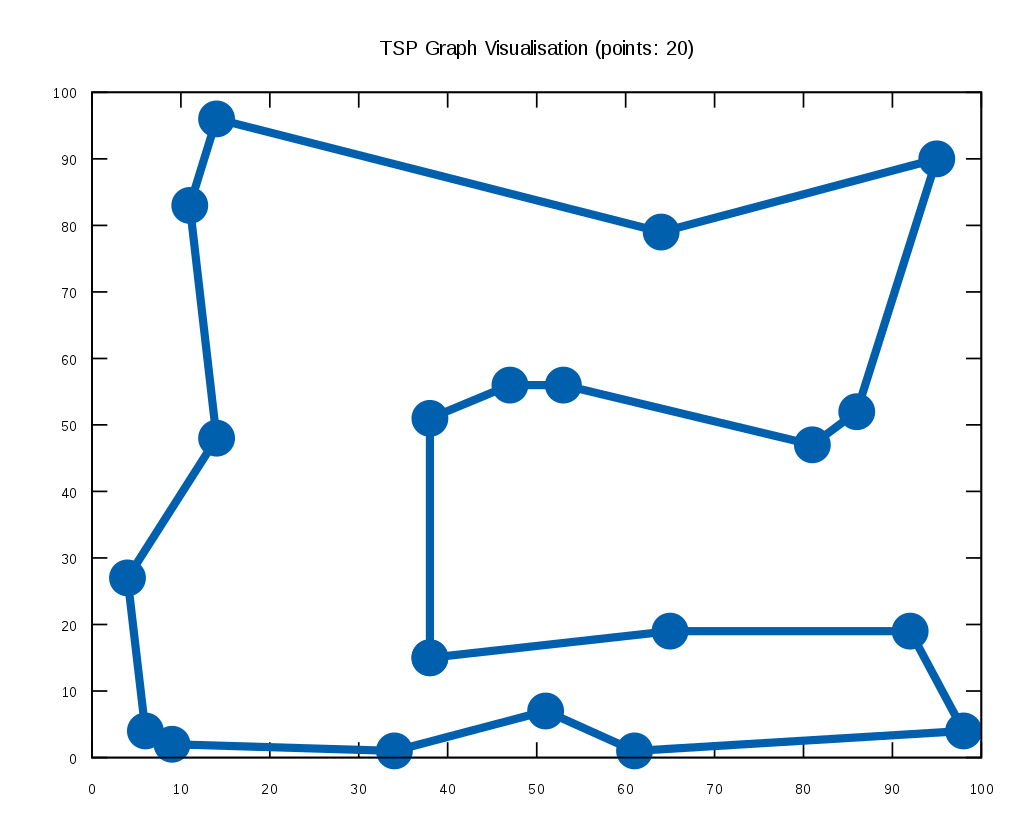
\includegraphics[width=400pt]{images/gnuplot_sample.png}
	\caption{Ausgabe von Gnuplot}
	\label{fig:gnuplot-sample}
\end{figure}

\section{Datenformat für Graphen und Populationen}
\label{sec:datenformat}

Wie bereits in \autoref{sec:visualisierung_graph} angedeutet, haben wir uns für das Datenformat Json entschieden, um Graphen und auch Populationen zu speichern. Json bietet gerade im Vergleich zu XML den Vorteil, dass die Syntax einfacher ist. Zudem erwies es sich als weniger umständlich ein Objekt in eine Json Repräsentation zu serialisieren oder eine Json Zeichenkette in ein Objekt umzuwandeln.

\chapter{Auswertung}
\label{chap:auswertung}

Im Rahmen dieses Projekts wurde der hier entwickelte und implementierte genetische Algorithmus auf seine Performanz untersucht. Hierbei stehen vor allem die Ergebnis- und Leistungsunterschiede die durch die Parallelisierung entstehen im Vordergrund.\\
Hierzu wurde der Algorithmus unter verschiedenen Szenarien getestet, welche in \autoref{sec:szenarien} vorgestellt werden.\\
Während dieser Tests wurden Metriken zur Leistungsanalyse erfasst und zu einem späteren Zeitpunkt ebenfalls ausgewertet. Eine ausführliche Beschreibung dieser Metriken wird in \autoref{sec:metriken} bereitgestellt.\\
Im letzten Abschnitt, \autoref{sec:ergebnisse}, werden die erfassten und ausgewerteten Daten vorgestellt und deren Interpretation erörtert.

\section{Szenarien}
\label{sec:szenarien}

In den Tests wurden insgesamt vier Szenarien betrachtet, um die Auswirkung der Parallelisierung auf die Ergebnisqualität zu untersuchen.

\begin{longtable}{p{5cm} p{7cm}}
\textbf{Szenario 1} & 1 Prozess auf 1 Maschine\\
\textbf{Szenario 2} & 8 Prozesse auf 1 Maschine\\
\textbf{Szenario 3} & 40 Prozesse auf 10 Maschinen\\
\textbf{Szenario 4} & 80 Prozesse auf 10 Maschinen
\end{longtable}

Alle diese Szenarien unterliegen den folgenden Rahmenbedingungen.

\begin{longtable}{ p{5cm} p{7cm} }
\textbf{Durchläufe} & 100\\
\textbf{Zeitbeschränkung} & 02:30 Minuten\\
\textbf{Population} & 50.000\\
\textbf{Größe des Graphen} & 500 Knoten\\
\end{longtable}

Ein Durchlauf ist hierbei genau ein Versuch des Algorithmus das TSP zu lösen. Nach einem Durchlauf verliert der Algorithmus alle gewonnen Kenntnisse über das Problem und startet in einem erneuten Durchlauf mit zufällig generierten Individuen.\\
Die Zeitbeschränkung gibt an wie lange der Algorithmus in einem Durchlauf Zeit hat, um das Problem zu bearbeiten.\\
Die Populationsgröße gibt an wie viele Individuen in einem einzelnen Durchlauf verwendet werden. Im Falle von parallelisierten Szenarien mit mehr als 1 Prozess wurde die Population gleichmäßig auf alle Prozesse aufgeteilt.\\
Schlussendlich gibt die Größe des Graphen an, wie viele Knoten der Graph beinhaltet und ist damit ein Komplexitätsmaß für das gestellte Problem. Der verwendete Graph ist in \autoref{fig:anwendung-graph} zu sehen.

\begin{figure}[ht]
  	\centering
	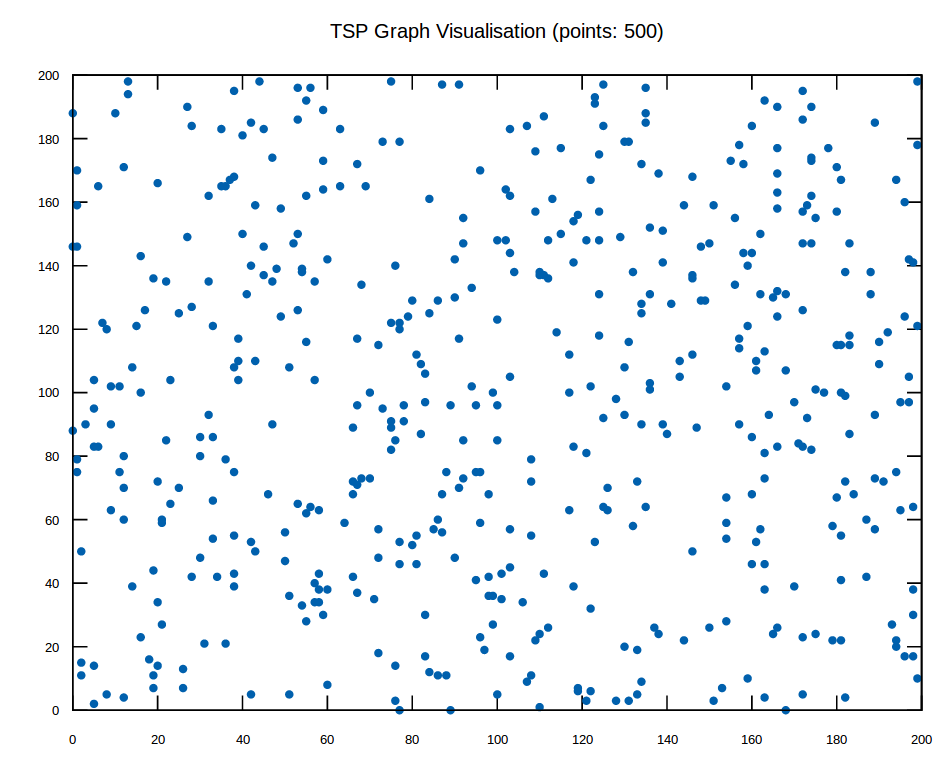
\includegraphics[width=400pt]{images/graph_01.png}
	\caption{Im Test verwendeter Graph}
	\label{fig:anwendung-graph}
\end{figure}

In diesem Graphen gibt es $1.220136826 * 10^{1131}$ Lösungsmöglichkeiten.

\section{Metriken}
\label{sec:metriken}

Die Leistung der Parallelisierung wurde anhand der folgenden vier Metriken gemessen:

\begin{longtable}{p{4.5cm} p{8.5cm}}
\textbf{Distanz pro Generation} & Für jede Generation wird der Distanzwert der besten Lösung über alle Durchläufe gemittelt. Hierdurch ergibt sich ein Maß dafür, ob sich verteilte Populationen pro Generation genauso verhalten wie eine einzelne große Population oder ob es in den Ergebnissen zur gleichen Generation gravierende Unterschiede gibt. Außerdem lässt sich zeigen, dass die Lösungen gegen einen bestimmten Wert konvergieren.\\
 & \\
\textbf{Enddistanz} & Über alle Durchläufe hinweg wird der Durchschnitt der Distanz der besten Lösung, die am Ende des jeweiligen Durchlaufs vorliegt, berechnet. Dies gibt ein Maß dafür wie gut die Lösungsqualität ist, die der Algorithmus in der gegebenen Zeit erreichen kann. Außerdem bietet diese Metrik die Möglichkeit die Peformanzunterschiede (welche Qualität kann in der gegebenen Zeit erreicht werden?) zwischen eines nebenläufigen und eines nicht nebenläufigen Szenarios zu untersuchen.\\
 & \\
\textbf{Anzahl der Generationen} & Hierbei wird der Durchschnitt der berechneten Generationen pro Durchlauf berechnet. Mit dieser Metrik lässt sich feststellen, inwiefern parallelisierte Szenarien schneller arbeiten, indem sie mehr Generationen in der selben Zeit berechnen können. \\
 & \\
\textbf{Zeit pro Generation} & Über alle Durchläufe hinweg wird die Zeit, die zur Berechnung einer einzigen Generation benötigt wurde, gemittelt. Dies stellt zwar den Umkehrschluss zur \textit{Anzahl der Generationen} dar, jedoch lässt sich mittels der Standardabweichung mit dieser Metrik feststellen wie konstant die einzelnen Szenarien ihre Performanz aufrechterhalten konnten.
\end{longtable}

\section{Ergebnisse}
\label{sec:ergebnisse}

Die im oben beschriebenen Test erfassten Daten wurden aufbereitet und werden in Form von Grafiken vorgestellt. Hierbei werden in den Balkendiagrammen die Durchschnittswerte durch die blauen Balken repräsentiert und die orangenen Markierungen geben die Standardabweichung der gemittelten Werte an.\absatz
\autoref{fig:dist-per-gen} zeigt die durchschnittliche Distanz pro Generation für jedes Szenario.

\begin{figure}[ht]
  	\centering
	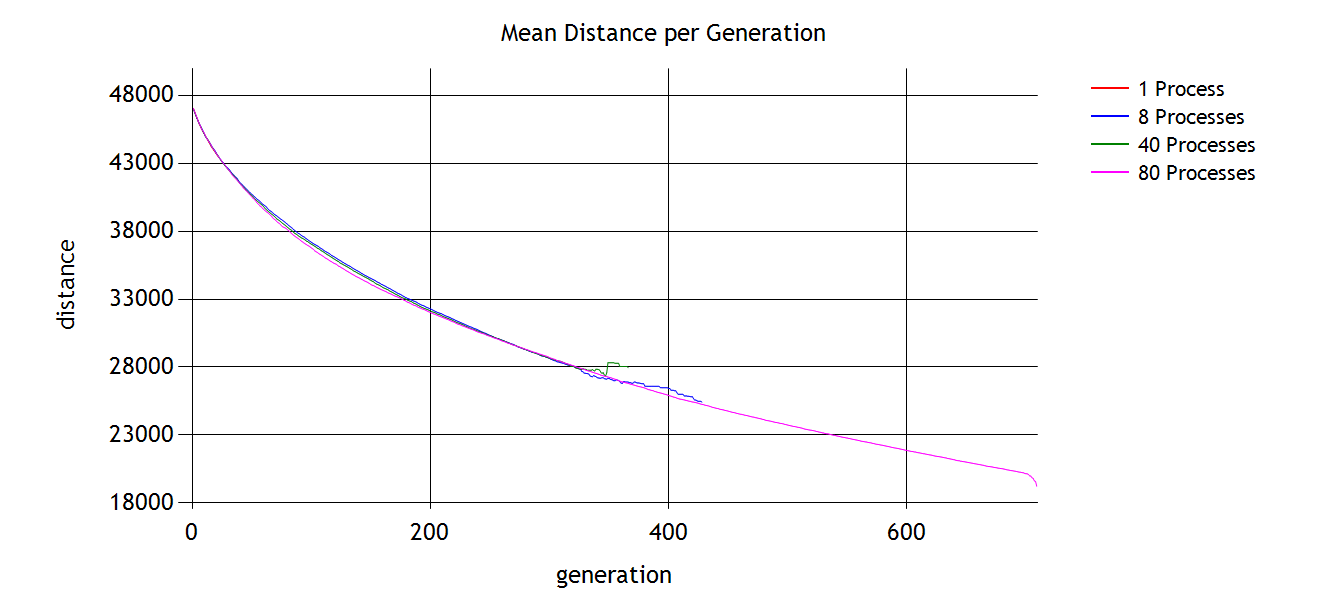
\includegraphics[width=400pt]{images/data_01_dist_per_gen.png}
	\caption{Durchschnittliche Distanz pro Generation je Szenario}
	\label{fig:dist-per-gen}
\end{figure}

Hierbei ist zu sehen, dass die Ergebnisse verschiedener Szenarien innerhalb derselben Generation kaum voneinander abweichen. Dies spricht für die in \autoref{subsec:exchange} aufgestellte Behauptung, dass sich eine verteilte Population in einer parallelisierten Anwendung näherungsweise wie eine einzelne Population verhält und als solche betrachtet werden kann.\\
Weiterhin ist zu sehen, dass die Kurve der \textit{80 Prozesse} gegen einen Wert konvergiert. Der abwärts Knick am Ende des Graphen deutet jedoch darauf hin, dass der Algorithmus hier nicht gegen die optimale Lösung konvergiert. Würde man dem Algorithmus mehr Zeit und eine größere Population zur Verfügung stellen könnte er noch bessere Lösungen finden.\absatz
In \autoref{fig:final-dist} wird der Durchschnitt der jeweils besten Lösung jedes Durchlaufs dargestellt.
\pagebreak

\begin{figure}[ht]
  	\centering
	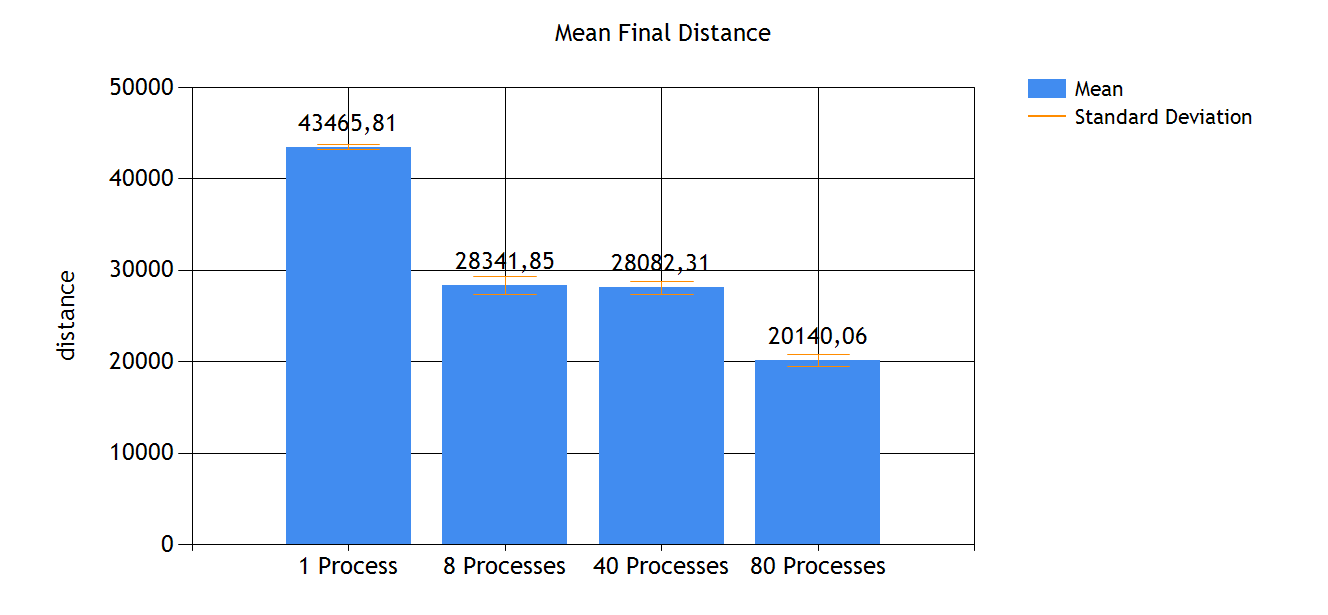
\includegraphics[width=400pt]{images/data_02_final_dist.png}
	\caption{Durchschnittliche Enddistanz pro Durchlauf}
	\label{fig:final-dist}
\end{figure}

Hierbei ist gut zu sehen, dass sich die Parallelisierung in Hinblick auf die Ergebnisqualität auszahlt. Die mit \textit{80 Prozessen} berechnete Distanz ist weniger als halb so groß als diejenige von nur \textit{1 Prozess}, wodurch sich die Ergebnisqualität mehr als verdoppelt hat.\\
Auffällig ist jedoch der geringe Unterschied zwischen \textit{8 Prozessen} und \textit{40 Prozessen}. Dies lässt sich jedoch damit erklären, dass sämtliche Prozesse in Szenario 2 auf demselben Rechner ausgeführt werden. In Szenario 3 hingegen werden die 40 Prozesse auf 10 Rechner verteilt, wodurch ein Netzwerk Overhead entsteht. Bei \textit{40 Prozessen} ist der Vorteil von zusätzlichen Prozesse noch nicht groß genug, um den Netzwerk Overhead auszugleichen. Jedoch zeigt sich, dass bei weiterer Erhöhung der Prozessanzahl (siehe \textit{80 Prozesse}) die Ergebnisqualität weiter zunimmt.\absatz
In der folgenden \autoref{fig:gen-count} wird die durchschnittliche Anzahl der berechneten Generationen in jedem Szenario dargestellt.
\pagebreak
\begin{figure}[ht]
  	\centering
	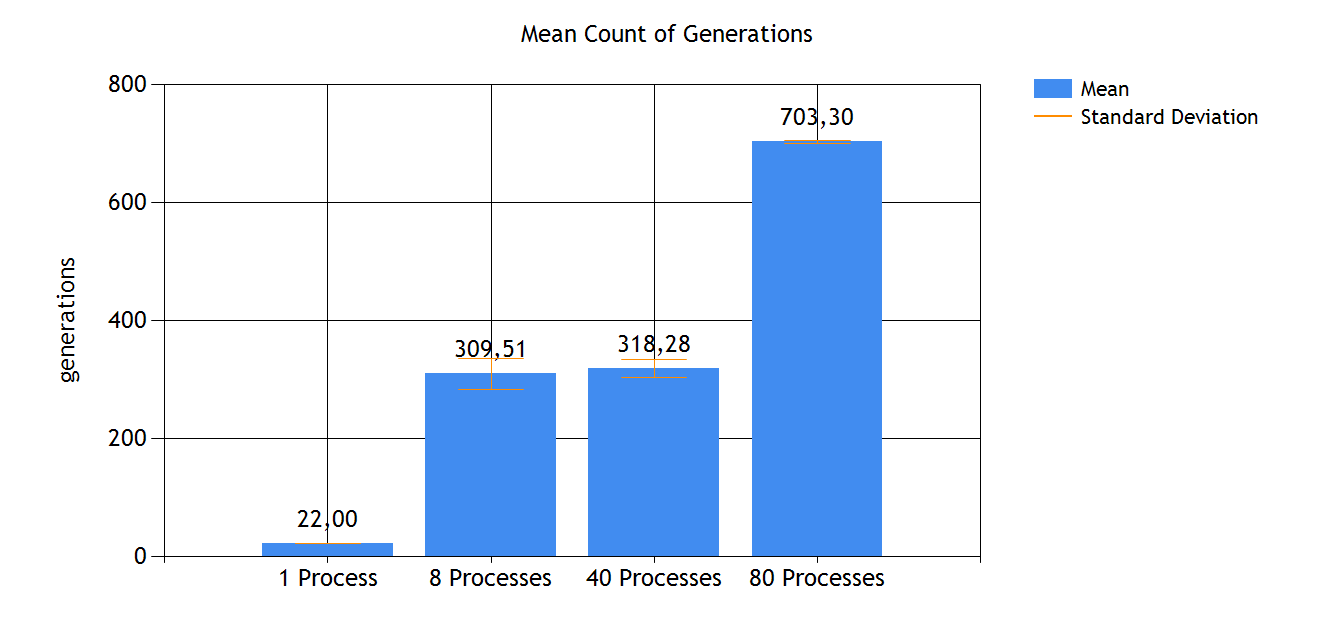
\includegraphics[width=400pt]{images/data_03_gen_count.png}
	\caption{Durchschnittliche Anzahl berechneter Generation je Szenario}
	\label{fig:gen-count}
\end{figure}

Hier zeigt sich, dass ein einzelner Prozess deutlich weniger Generationen in der gleichen Zeit berechnen kann als eine parallelisierte Variante. \textit{80 Prozesse} schaffen hierbei beinahe 32 mal so viele Generationen als \textit{1 Prozess}. Damit arbeitet Szenario 4 deutlich schneller. Vergleicht man dieses Ergebnis außerdem mit dem Ergebnis aus \autoref{fig:final-dist} so zeigt sich, dass die Ergebnisqualität sich keineswegs proportional zur Performanz verhält. So arbeiten \textit{80 Prozesse} zwar 32 mal so schnell als \textit{1 Prozess}, jedoch erreichen sie damit gerade mal ein doppelt so gutes Ergebnis.\\
Auch hier zeigt sich das zuvor festgestellte Phänomen, dass \textit{40 Prozesse} etwa gleiche Ergebnisse wie \textit{8 Prozesse} erzielen. Wieder ist der Grund hierfür, dass der Netzwerk Overhead mit \textit{40 Prozessen} nicht ausgeglichen werden kann.\absatz
Zuletzt betrachten wir die durchschnittliche Berechnungszeit pro Generation in \autoref{fig:time-per-gen}.
\pagebreak
\begin{figure}[ht]
  	\centering
	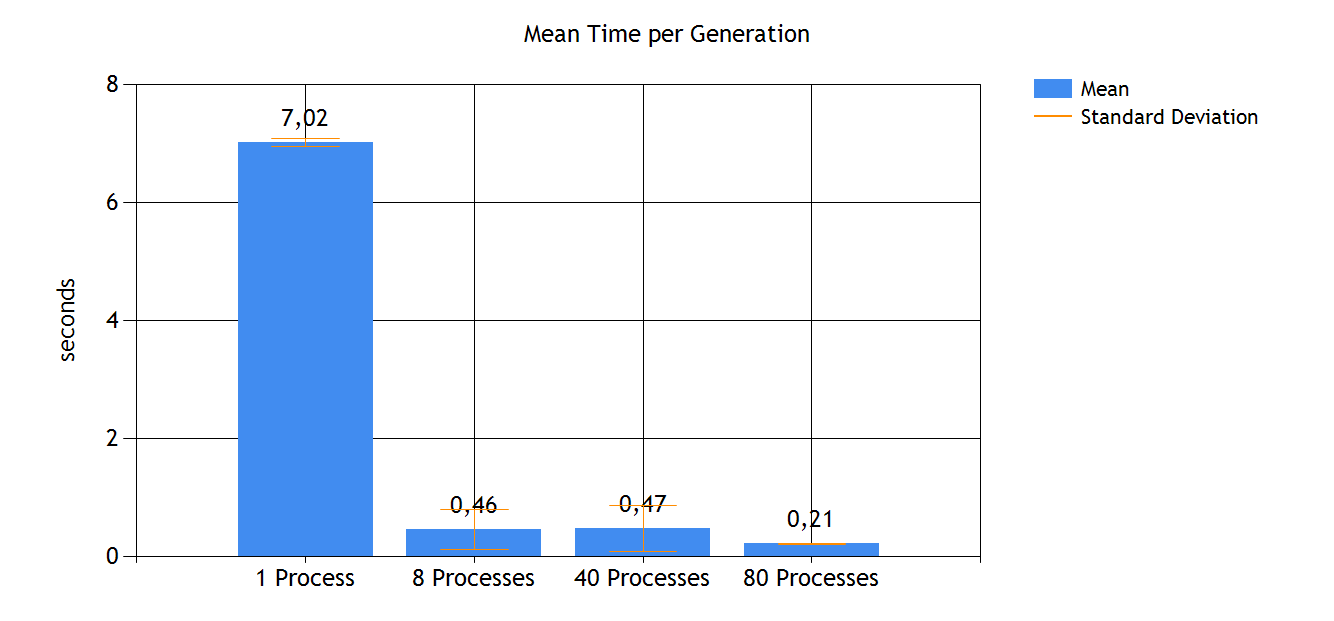
\includegraphics[width=400pt]{images/data_04_time_per_gen.png}
	\caption{Durchschnittliche Berechnungszeit einer Generation je Szenario}
	\label{fig:time-per-gen}
\end{figure}

Auch hier wird ersichtlich, dass in einem parallelisierten Szenario Generationen deutlich schneller verarbeitet werden können. Da in Szenario 1 ein einzelner Prozess eine Population von 50.000 Individuen berechnen muss dauert eine Generation auch etwa 32 mal so lange wie in Szenario 4, bei dem jeder einzelne Prozess nur eine Population von 625 Individuen pro Generation berechnen muss.\\
Hier fällt jedoch auf, dass \textit{8 Prozesse} und \textit{40 Prozesse} eine höhere Standardabweichung haben als \textit{1 Prozess}. Damit ist die Ausführungszeit pro Generation deutlich unstetiger, was durch den Netzwerk Overhead und die Prozesskommunikation erklärt werden kann. Falls ein Prozess aufgrund von Scheduling durch das Betriebssystem etwas länger benötigt als ein anderer, so muss der schnellere auf den langsameren warten. Das Ganze verschärft sich in Szenario 3 weiter, da dort noch Verzögerungen durch das Netzwerk hinzukommen und die verwendeten Rechner nicht vollständig identisch sind (siehe \autoref{chap:testumgebung}) und somit schnellere Prozesse wieder auf langsamere warten müssen, um Individuen austauschen zu können.

\chapter{Ausblick}
\label{chap:ausblick}

Wie gezeigt wurde, ist das Travelling Salesman Problem bestens geeignet, um es mithilfe eines genetischen Algorithmus zu parallelisieren. Mit dem hier vorgestellten Ansatz, wird die optimale Lösung höchstens zufällig erreicht und die Endergebnisse sind mit der aktuellen Implementierung und den gewählten Startparametern lediglich hinreichend gut. Je nach den Rahmenbedingungen, wie der zur Verfügung stehenden Zeit, lassen sich möglicherweise noch bessere Ergebnisse erzielen. Eine Möglichkeit besteht darin, die Werte der folgenden Parameter für den Algorithmus weiter zu optimieren:

\begin{itemize}
\item Anzahl der zu berechnenden Generationen (falls keine Zeitbegrenzung gesetzt wird)
\item Populationsgröße
\item Anteil der Elite, die in die nächste Generation übernommen wird
\item Mutationswahrscheinlichkeit
\item Fitnessexponent (wie viel besser sich Individuen mit einer hohen Fitness fortpflanzen)
\item Austauschrate (zwischen getrennten Populationen)
\end{itemize}

Weiteres Verbesserungspotential liegt zudem darin, den genetischen Algorithmus mit anderen Algorithmen zu kombinieren. Anbieten würde sich beispielsweise die Auflösung von sich kreuzenden Kanten, da diese ein Indiz dafür sind, dass es sich noch nicht um eine hinreichend gute Lösung handelt.\\
Interessant wäre zudem ein Leistungsvergleich mit anderen Algorithmen, die ebenfalls nicht vordergründig die optimale Lösung liefern, deren Ziel aber ebenfalls eine hinreichend gute Näherung ist.

\clearpage
\pagenumbering{Roman}
\lstlistoflistings
\addcontentsline{toc}{chapter}{\lstlistlistingname}
\listoffigures
\listoftables
\bibliographystyle{plain}
\bibliography{literature}

\end{document}